\PassOptionsToPackage{table}{xcolor}
\documentclass[review,onefignum,onetabnum,a4paper]{siamart190516}
\pdfoutput=1
\overfullrule=0pt

%------------------------------------------------------------------------------
% Header
%------------------------------------------------------------------------------
\usepackage[utf8]{inputenc}
\usepackage[english]{babel}
\usepackage{amsmath, amssymb, gensymb, physics, upgreek, siunitx, bbm}
\usepackage{tikz, pgfplots, graphicx, epstopdf, float, hyperref, xspace}
\usepackage[caption=false]{subfig}
\usepackage{enumitem, verbatim, listings}
\usepackage{mathtools, stmaryrd}
\usepackage{booktabs, array, ragged2e}
\usepackage[export]{adjustbox}
\usepackage{cleveref}
\usepackage{todonotes}

\sisetup{table-number-alignment=center, exponent-product=\times}
\newcommand{\crefrangeconjunction}{--}

\usetikzlibrary{trees, cd, babel}
\graphicspath{{./figures}}
\epstopdfsetup{outdir=./}

\lstset{basicstyle=\footnotesize\ttfamily}

\definecolor{paired1}{HTML}{a6cee3}
\definecolor{paired2}{HTML}{1f78b4}
\definecolor{paired3}{HTML}{b2df8a}
\definecolor{paired4}{HTML}{33a02c}
\definecolor{paired5}{HTML}{fb9a99}
\definecolor{paired6}{HTML}{e31a1c}
\definecolor{paired7}{HTML}{fdbf6f}
\definecolor{paired8}{HTML}{ff7f00}
\definecolor{paired9}{HTML}{cab2d6}
\definecolor{paired10}{HTML}{6a3d9a}

\hypersetup{
    colorlinks,
    linkcolor={red!50!black},
    citecolor={blue!50!black},
    urlcolor={blue!80!black}
}

\pgfplotsset{
  log x ticks with fixed point/.style={
      xticklabel={
        \pgfkeys{/pgf/fpu=true}
        \pgfmathparse{exp(\tick)}%
        \pgfmathprintnumber[fixed relative, precision=3]{\pgfmathresult}
        \pgfkeys{/pgf/fpu=false}
      }
  },
  log y ticks with fixed point/.style={
      yticklabel={
        \pgfkeys{/pgf/fpu=true}
        \pgfmathparse{exp(\tick)}%
        \pgfmathprintnumber[fixed relative, precision=3]{\pgfmathresult}
        \pgfkeys{/pgf/fpu=false}
      }
  }
}

% Classic symbols
\newcommand{\reals}{\mathbb{R}}
\newcommand{\integers}{\mathbb{Z}}
\newcommand{\dx}{\,\d\mathbf{x}}
\newcommand{\md}{\,\d}
\newcommand{\bigo}[1]{\mathcal{O}(#1)}
\DeclareMathOperator*{\argmin}{arg\,min}
\DeclareMathOperator*{\union}{\cup}


\let\grad\undefined
\let\curl\undefined
\let\div\undefined
\let\nullop\undefined
\let\d\undefined
\let\tr\undefined
\DeclareMathOperator{\grad}{grad}
\DeclareMathOperator{\curl}{curl}
\DeclareMathOperator{\div}{div}
\DeclareMathOperator{\nullop}{null}
\DeclareMathOperator{\d}{d}
\DeclareMathOperator{\tr}{tr}
\DeclareMathOperator{\Exists}{\exists}
\DeclareMathOperator{\Forall}{\forall}

\DeclareMathOperator{\refgrad}{\widehat{\grad}}
\DeclareMathOperator{\refcurl}{\widehat{\curl}}
\DeclareMathOperator{\refdiv}{\widehat{\div}}

\newcommand{\Hgrad}{H(\grad)}
\newcommand{\Hcurl}{H(\curl)}
\newcommand{\Hdiv}{H(\div)}
\newcommand{\Ltwo}{L^2}


\newcommand{\mesh}{\mathcal{T}_h}
\newcommand{\skeleton}{\mathcal{E}_h}
\newcommand{\refline}{\hat{\mathcal{I}}}
\newcommand{\jac}{\mathrm{D}F}
\newcommand{\pullback}{\mathcal{F}}
\newcommand{\betah}{\tilde{\beta}}

% Vector notation
\renewcommand{\vec}[1]{\mathbf{#1}}
\newcommand{\uvec}[1]{\mathbf{\hat{#1}}}
\newcommand{\conj}[1]{{\overline{#1}}}
\DeclareMathOperator{\blockdiag}{blockdiag}
\DeclareMathOperator{\diag}{diag}
\DeclareMathOperator{\spn}{span}
\DeclareMathOperator{\vecop}{vec}
\newcommand{\eye}{{\mathbb{I}}}
\newcommand{\kron}{\otimes}
\newcommand{\jump}[1]{\left\llbracket #1 \right\rrbracket}
\newcommand{\avg}[1]{\left\{ #1 \right\}}
\newcommand{\broken}[1]{\tilde{#1}}


\newcommand{\be}{\vec{e}}
\newcommand{\bu}{\vec{u}}
\newcommand{\bn}{\vec{n}}
\newcommand{\bt}{\vec{t}}
\newcommand{\bm}{\vec{m}}
\newcommand{\bv}{\vec{v}}
\renewcommand{\bf}{\vec{f}}
\newcommand{\bq}{\vec{q}}
\newcommand{\br}{\vec{r}}
\newcommand{\bx}{\vec{x}}
\newcommand{\bw}{\vec{w}}
\newcommand{\by}{\vec{y}}
\newcommand{\bz}{\vec{z}}
\newcommand{\bB}{\vec{B}}
\newcommand{\bC}{\vec{C}}
\newcommand{\bE}{\vec{E}}
\newcommand{\bF}{\vec{F}}
\newcommand{\bJ}{\vec{J}}
\newcommand{\bP}{\vec{P}}
\newcommand{\bT}{\vec{T}}
\newcommand{\bX}{\vec{X}}

\newcommand{\ub}{\underline{b}}
\newcommand{\uc}{\underline{c}}
\newcommand{\ue}{\underline{e}}
\newcommand{\uf}{\underline{f}}
\newcommand{\ug}{\underline{g}}
\newcommand{\up}{\underline{p}}
\newcommand{\uq}{\underline{q}}
\newcommand{\ur}{\underline{r}}
\newcommand{\uu}{\underline{u}}
\newcommand{\uv}{\underline{v}}
\newcommand{\uw}{\underline{w}}
\newcommand{\ux}{\underline{x}}
\newcommand{\uy}{\underline{y}}
\newcommand{\uz}{\underline{z}}
\newcommand{\ut}{\underline{t}}
\newcommand{\ulambda}{\underline{\lambda}}

\newcommand{\uB}{\underline{B}}
\newcommand{\ubb}{\underline{\vec{b}}}
\newcommand{\ubq}{\underline{\vec{q}}}
\newcommand{\ubu}{\underline{\vec{u}}}
\newcommand{\ubv}{\underline{\vec{v}}}
\newcommand{\ubf}{\underline{\vec{f}}}
\newcommand{\ubg}{\underline{\vec{g}}}

\newcommand{\xhat}{\hat{x}}
\newcommand{\rhat}{\hat{r}}
\newcommand{\shat}{\hat{s}}
\newcommand{\Khat}{\hat{K}}
\newcommand{\Bhat}{\hat{B}}
\newcommand{\Ahat}{\hat{A}}
\newcommand{\Dhat}{\hat{D}}
\newcommand{\Shat}{\hat{S}}
\newcommand{\Ghat}{\hat{G}}

\renewcommand{\P}{\mathrm{P}}
\newcommand{\DP}{\mathrm{DP}}
\newcommand{\CG}{\mathrm{CG}}
\newcommand{\DG}{\mathrm{DG}}
\newcommand{\Ned}{\mathrm{Ned}^{1}}
\newcommand{\RT}{\mathrm{RT}}
\newcommand{\BDM}{\mathrm{BDM}}
\newcommand{\NedTwo}{\mathrm{Ned}^{2}}


\newcommand{\Nedelec}{Ned\'el\'ec~}

\newcommand{\pef}[1]{\todo[inline,color=blue!40]{PEF: #1}}

%\newtheorem{theorem}{Theorem}
\newtheorem{remark}{Remark}


%------------------------------------------------------------------------------
% Document
%------------------------------------------------------------------------------

\title{
   Fast solvers for the high-order FEM simplicial de Rham complex
\thanks{Submitted to the editors July XX, 2024.
      \funding{
         PDB and PEF were supported by EPSRC grant EP/W026260/1.
      }
   }
}

\author{Pablo D.\ Brubeck\thanks{
Mathematical Institute,
University of Oxford,
Oxford, UK (\email{brubeckmarti@maths.ox.ac.uk})
%\orcid{0000-0002-3824-0080}
}
\and Patrick E.\ Farrell\thanks{
Mathematical Institute,
University of Oxford,
Oxford, UK (\email{patrick.farrell@maths.ox.ac.uk})
%\orcid{0000-0002-1241-7060}
}
\and Robert C.\ Kirby\thanks{
Department of Mathematics,
Baylor University,
Waco, TX, USA (\email{robert\_kirby@baylor.edu})
%\orcid{0000-0002-1241-7060}
}
}

\headers{Patch solvers for simplicial $p$-FEM}{P.~D.~Brubeck and P.~E.~Farrell and R.~C.~Kirby}

\begin{document}

\numberwithin{equation}{section}
\maketitle

\begin{abstract}
We present new high-order finite elements discretizing the $L^2$ de Rham
complex on triangular and tetrahedral meshes. The finite elements discretize
the same spaces as usual, but with different basis functions. They allow for
fast linear solvers based on static condensation and space decomposition
methods. The new elements build upon the definition of degrees of freedom
given in [L.~Demkowicz, P.~Monk, L.~Vardapetyan, and W.~Rachowicz,
Comput.~Math.~Appl.,
39(7-8) (2000), pp.~29--38], and consist of integral moments
on an equilateral reference simplex with respect to a numerically computed
polynomial basis that is orthogonal in both the $L^2$- and
$H(\mathrm{d})$-inner products ($\mathrm{d} \in \{\mathrm{grad},
\mathrm{curl}, \mathrm{div}\}$). 
On the reference equilateral simplex, the
resulting stiffness matrix has diagonal interior block, and does not couple
together the interior and interface degrees of freedom. Thus, on the
reference simplex, the Schur complement resulting from the elimination of
interior degrees of freedom is simply the interface block itself. This
sparsity is not preserved on arbitrary cells mapped from the reference cell.
Nevertheless, the interior-interface coupling is weak because it is only
induced by the geometric transformation. We devise a preconditioning
strategy by neglecting the interior-interface coupling. We precondition the
interface Schur complement with the interface block, and simply apply
point-Jacobi to precondition the interior block. The combination of this
approach with a space decomposition method on small subdomains constructed
around vertices and edges allows us to efficiently solve the
canonical Riesz maps in $H(\mathrm{grad})$, $H(\mathrm{curl})$, and
$H(\mathrm{div})$, at very high order. We empirically demonstrate iteration
counts that are robust with respect to the polynomial degree, with a computational complexity of $\mathcal{O}(p^{6})$ flops in three dimensions
instead of the na\"ive $\mathcal{O}(p^{9})$.
\end{abstract}

\begin{keywords}
   preconditioning, de Rham complex, simplex, high-order, additive Schwarz
\end{keywords}

\begin{AMS}
   65F08, 65N35, 65N55
\end{AMS}

%\begin{DOI}
%10.1137/21XXXXXXX
%\end{DOI}

\section{Introduction} \label{sec:introduction}

High-order finite element discretizations have very attractive properties, such as rapid convergence and higher arithmetic intensity. However, their implementation requires great care, as na\"ive approaches to operator evaluation and linear system solution can scale badly in terms of memory and floating-point operations (flops) as the polynomial degree $p$ increases. On a single $d$-dimensional cell, the number of degrees of freedom scales like $p^d$; computing the $\mathcal{O}(p^{2d})$ entries of a dense stiffness matrix with standard Lagrange-type elements would cost $\mathcal{O}(p^{3d})$ flops. Making high-order discretizations competitive therefore requires better algorithms.

For tensor-product cells (quadrilaterals and hexahedra), a tensor-product basis naturally exposes the required structure to decouple multidimensional problems into a sequence of one-dimensional problems, reducing computational cost and storage. For example, the sum-factorization assembly strategy enables fast matrix-free operator evaluation in $\mathcal{O}(p^{d+1})$ operations and $\mathcal{O}(p^{d})$ storage~\cite{orszag80}, and the fast diagonlization method (FDM) addresses the solution of separable problems on structured domains with the same complexities~\cite{lynch64}. The previous work of the first two authors employing FDM-inspired finite element bases with suitable space decompositions yields the solution of certain separable and non-separable problems on unstructured domains with the same complexities~\cite{brubeck22,brubeck24}.

Achieving similar computational complexities on simplices is more challenging. Bernstein--B\'ezier expansions enable sum-factorized matrix-free operator evaluation in $\mathcal{O}(p^{d+1})$ operations and $\mathcal{O}(p^{d})$ storage~\cite{ainsworth11}, but there is no known analogue of an FDM approach that solves the linear systems arising from separable problems with these complexities. This manuscript makes a step towards addressing this challenge.

The essential idea of our approach is to devise new finite elements for the $L^2$ de Rham complex that promote sparsity in the reference
element, in a similar spirit to~\cite{brubeck24}. On the reference cell, the interior and interface degrees of freedom are decoupled; on generally mapped cells, they are only coupled by the geometric transformation, and hence for suitably-shaped cells the coupling is weak. This increases the efficiency of block preconditioning strategies that decouple the interface and interior degrees of freedom. This reference cell sparsity is achieved by employing the framework of Demkowicz et al.~\cite{demkowicz00}, by making a clever choice for bases of bubble spaces that arise in the construction of the degrees of freedom. The bases for the bubble spaces are constructed by solving a handful of offline eigenproblems on the reference cell for each polynomial degree $p$. This combination of finite elements and block preconditioning strategy solves the Riesz maps of the $L^2$ de Rham complex in $\mathcal{O}(p^{3(d-1)})$ operations and $\mathcal{O}(p^{2(d-1)})$ storage; worse than the optimal complexities achieved on tensor-product cells, but orders of magnitude better than previously available approaches [FIXME is this true].

Main challenges, motivations
\begin{itemize}
\item In high-order FEM, the curse of dimensionality affects operator
   evaluation and relaxation methods in multigrid and domain-decomposition.  
\item For tensor product cells,
   a tensor product basis will expose the structure to decouple the
   multidimensional problems into a sequence of one-dimensional problems.
   Sum-factorization enables fast operator evaluation, and the fast
   diagonalization method addresses the efficient solution of problems
   structured subdomains.  On unstructured subdomains, an optimal strategy
   using static condensation with FDM bases was proposed in our previous
   work.
\item For simplices, Bernstein--Bezier expansions enable sum-factorized
   operator evaluation, but there is no knowledge of a basis transformation
   that can diagonalize a problem on any structured or unstructured subdomain.
\end{itemize}


Other approaches
\begin{itemize}
\item Low-order-refined preconditioning, not fully understood/far from optimal.
\item Sparse hierarchical bases from Beuchler \& Schoberl constructed from integrated Jacobi polynomials. 
   These bases still couple interior DOFs, making static condensation difficult.
\end{itemize}


Our approach, main solver design ingredients:
\begin{itemize}
\item Construction of degrees of freedom that promote sparsity in the reference element, 
   which in turn increases the efficiency of block preconditioners/decoupling strategies. The key idea is
      to use the degrees of freedom proposed by Demkowicz with eigenbases for the space of bubbles on each subentity.
\item Construction of space decompositions around small subdomains constructed around vertices and edges.
\end{itemize}



\section{Sparsity-promoting discretizations} \label{sec:dofs}

We discretize the $\Ltwo$ de Rham complex on triangular and tetrahedral meshes with finite element subcomplexes of the first and second kinds.

\begin{figure}[htbp] 
\centering
\begin{tikzcd}
  \CG_p \arrow[r, "\grad"] & \Ned_p \arrow[r, "\curl"] & 
   \RT_p \arrow[r, "\div"] & \DG_{p-1} \\
  \Hgrad \arrow[r, "\grad"] \arrow[u] \arrow[d]  & \Hcurl \arrow[r, "\curl"]
  \arrow[d] \arrow[u] & \Hdiv \arrow[r, "\div"] \arrow[u] \arrow[d] & \Ltwo \arrow[u] \arrow[d] \\
   \CG_p \arrow[r, "\grad"] & \NedTwo_{p-1} \arrow[r, "\curl"] & 
   \BDM_{p-2} \arrow[r, "\div"] & \DG_{p-3}
\end{tikzcd}
\caption{The $\Ltwo$ de Rham complex (middle), and the finite element subcomplexes of the first (above) and second kinds (below).}
\end{figure}
\pef{Fix vertical alignment}

For each finite element subcomplex built on a mesh $\mesh$ of a domain $\Omega \subset \mathbb{R}^d$, we denote the spaces discretizing $k$-forms $H\Lambda^k(\Omega)$ with polynomial degree $p$ as $X^k_p(\mesh)$.
These are built from cellwise spaces via the standard pullback construction from a reference cell $\Khat$:
\begin{equation}
X^k_{h,p} = X^k_p(\mesh) = \{ v \in H\Lambda^k(\Omega): \Forall K \in \mesh \Exists \hat{v} \in X^k_p(\Khat) \text{ s.t.} \left.v\right|_K = \pullback^k_K(\hat{v}) \},
\end{equation}
where $\pullback^k_K$ denotes the appropriate pullback that preserves continuity of the traces of a $k$-form across cell facets.

We follow the definition of interpolation degrees of freedom from
Demkowicz et al.~\cite{demkowicz00} to construct dual bases that promote orthogonality in the
$\Ltwo(\Khat)$ and $H(\mathrm{d}, \Khat)$ inner products.
In the construction of the degrees of freedom we will employ bubble subspaces on a given mesh entity $S \subset \Khat$ with zero trace, defined as
\begin{equation}
B^k_p(S) \coloneqq \{v \in X^k_p(S): \tr v = 0 \text{ on } \partial S\}.
\end{equation}

Throughout we choose $\Khat$ to be an equilateral simplex, as this ...

\subsection{Sparsity-promoting basis for $\Hgrad$}

On $\Khat$ we discretize $\Hgrad$ with the space
\begin{equation}
X^0_{p}(\Khat) = \P_p(\Khat),
\end{equation}
where $\P_p(\Khat)$ is the space of polynomials of total degree less than or equal to $p$.
We define a basis for the dual of $X^0_p(\Khat)$ as
point evaluations at $V \in \text{vertices}(\Khat)$,
\begin{equation}
   \ell^V(v) = v(V),
\end{equation}
and for each sub-entity $S \in \text{edges}(\Khat) \union \text{faces}(\Khat) \union \text{interior}(\Khat)$
we take integral moments of surface gradients, 
\begin{equation}
   \ell^S_j(v) = (\grad_S\phi^S_j, \grad_S v)_{S},
\end{equation}
where $\grad_S$ is the tangential gradient on $S$,
and $\{\phi^S_j\}$ is a basis for $B^0_p(S)$
such that
\begin{equation} \label{eq:hgrad-fdm}
   (\grad_S\phi^S_j, \grad_S\phi^S_i)_{S} = \delta_{ij}, \quad
   (\phi^S_j, \phi^S_i)_{S} = \lambda_j\delta_{ij}.
\end{equation}
The eigenbases $\{\phi^S_j\}$ are numerically computed offline and only once 
on the reference interval, triangle, and tetrahedron.


\subsection{Sparsity-promoting basis for $\Hcurl$}

Recall the definition of the $\Hcurl$-conforming finite element spaces
\begin{equation}
   X^1_{p, p_E}(K) = \{v\in [\P_p(K)]^d : \tr v \in \P_{p_E}(E) \Forall E \in \text{edges}(K)  \}
\end{equation}
for $p_E=p-1$ we obtain the \Nedelec space of the first kind $\Ned_p(K)$, while
$p_E=p$ gives the \Nedelec space of the second kind $\NedTwo_p(K) = [\P_p(K)]^d$. 
These spaces enforce continuity of the tangential trace across mesh interfaces.


We define a basis for the dual of $X^1_{p, p_E}(K)$ as 
tangential moments along $E\in \text{edges}(\Khat)$,
\begin{equation}
   \ell^E_j(v) = (q_j, v\cdot \bt)_E, \quad q_j \in \P_{p_E}(E), 
\end{equation}
and for each sub-entity $S \in \text{faces}(\Khat) \cup \text{interior}(\Khat)$,
\begin{align}
   \ell^{S,0}_j(v) &= (\grad_S\phi^S_j, v)_{S}, \\
   \ell^{S,1}_j(v) &= (\curl_S\Phi^S_j, \curl_S v)_{S}, \label{eq:hcurl-interior-dofs}
\end{align}
where $\curl_S$ is the tangential curl on $S$,
$\{\phi^S_j\}$ are the $B^0_{p_S}(S)$ bases constructed in \eqref{eq:hgrad-fdm},
and $\{\curl_S\Phi^S_j\}$ is a basis for $\curl_S B^1_{p_S}(S)$
such that
\begin{equation} \label{eq:hcurl-fdm}
   (\curl_S\Phi^S_j, \curl_S\Phi^S_i)_{S} = \delta_{ij}, \quad
   (\Phi^S_j, \Phi^S_i)_{S} = \lambda_j\delta_{ij}.
\end{equation}


\subsection{Sparsity-promoting basis for $\Hdiv$}

Recall the definition of the $\Hdiv$-conforming finite element spaces
\begin{equation}
   X^2_{p, p_F}(K) = \{v\in [\P_p(K)]^d : \tr v \in \P_{p_F}(F) \Forall F \in \text{faces}(K)  \}
\end{equation}
for $p_F=p-1$ we obtain the Raviart--Thomas space $\RT_p(K)$, while
$p_F=p$ gives the Brezzi--Douglas--Marini space $\BDM_p(K) = [\P_p(K)]^d$. 
These spaces enforce continuity of the normal trace across mesh interfaces.

We define a basis for the dual of $X^2_{p, p_F}(K)$ as normal moments on $F\in
\text{faces}(\Khat)$,
\begin{equation}
   \ell^F_j(v) = (q_j, v\cdot \bn)_F, \quad q_j \in \P_{p_F}(F),
\end{equation}
and on the $\text{interior}(\Khat) = K$: 
\begin{align}
   \ell^{K,0}_j(v) &= (\curl\Phi^K_j, v)_{K}, \\
   \ell^{K,1}_j(v) &= (\div\Psi^K_j, \div v)_{K}, \label{eq:hdiv-interior-dofs}
\end{align}
where $\{\Phi^K_j\}$ are the $B^1_p(K)$ bases constructed in
\eqref{eq:hcurl-fdm}, and $\{\div\Psi^K_j\}$ is a basis for $\div B^2_p(K)$ such that
\begin{equation} \label{eq:hdiv-fdm}
   (\div\Psi^K_j, \div\Psi^K_i)_K = \delta_{ij}, \quad
   (\Psi^K_j, \Psi^K_i)_{K} = \lambda_j\delta_{ij}.
\end{equation}



\subsection{Generally-mapped elements}

On an equilateral simplex, the interior block of the mass and stiffness matrices
is fully diagonal, moreover the interior-interface blocks in the stiffness 
vanish for generally mapped elements.

The dual bases described above yield interior-orthogonal primal bases for $V^k_p(K)$ only
if $K$ is equilateral. For generally mapped triangles, the spectral equivalence constant of
a space decomposition that decouples the interior degrees of freedom should depend on how
far the element departs from being equilateral, i.e., the shape regularity parameter. 



\section{Design of preconditioners}




We follow 
the low-order space decompositions studied in \cite{arnold00}
and extend them to high-order with static-condensation.

For 0-forms we construct patches on vertex-stars,
\begin{equation}
   X^0_{h,p} = \left.X^0_{h,p}\right|_\mathcal{I} + X^0_{h,1} 
   + \sum_{v\in E^0(\mesh)} \left.\tilde{X}^0_{h,p}\right|_{\star v} 
\end{equation}

For 1-forms we construct edge-star patches
plus the gradient of vertex-star patches on 0-forms
\begin{equation}
   X^1_{h,p} = \left.X^1_{h,p}\right|_\mathcal{I} +  X^1_{h,1}
   + \sum_{e\in E^1(\mesh)} \left.\tilde{X}^1_{h,p}\right|_{\star e} 
   + \sum_{v\in E^0(\mesh)} \mathrm{d} \left.\tilde{X}^0_{h,p}\right|_{\star v} 
\end{equation}

For 2-forms we construct edge-star patches,
\begin{equation}
   X^2_{h,p} = \left.X^2_{h,p}\right|_\mathcal{I} +  X^2_{h,1} 
   + \sum_{e\in E^1(\mesh)} \left.\tilde{X}^2_{h,p}\right|_{\star e}. 
\end{equation}



\begin{figure}
\footnotesize
\centering
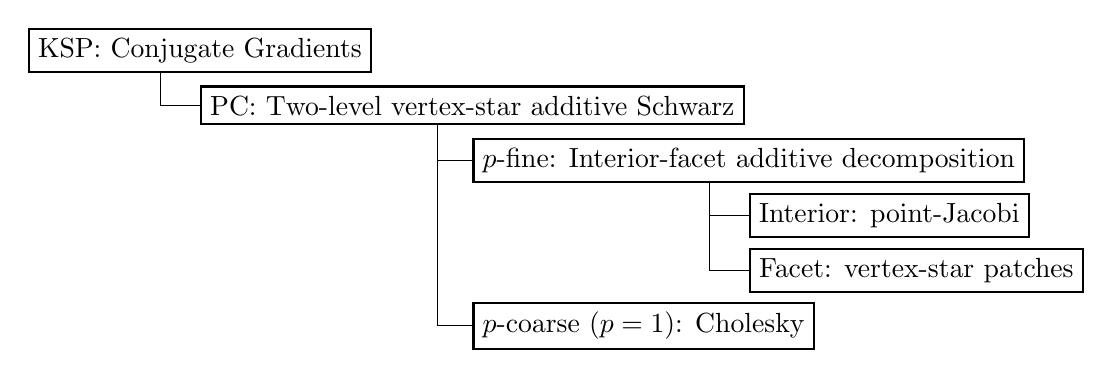
\begin{tikzpicture}[%
 every node/.style={draw=black, thick, anchor=west},
grow via three points={one child at (-0.0,-0.7) and
	two children at (0.0,-0.7) and (0.0,-1.4)},
edge from parent path={(\tikzparentnode.210) |- (\tikzchildnode.west)}]
\node {KSP: Conjugate Gradients}
   child {node {PC: Two-level vertex-star additive Schwarz}
   child {node {$p$-fine: Interior-facet additive decomposition}
      child {node {Interior: point-Jacobi}}
      child {node {Facet: vertex-star patches}}
   }
   child[missing]{}
   child[missing]{}
   child {node {$p$-coarse ($p=1$): Cholesky}
      %child {node {Relaxation: Hiptmair--Jacobi}}
      %child {node {$h$-coarse: Cholesky}}
   }
};
\end{tikzpicture}
\caption{Solver diagram for $\Hgrad$ using the interior-facet decomposition.}
\end{figure}


\section{Numerical results} \label{sec:results}

\subsection{Unit cube tests}
Here we want to address questions about $h$ and $p$ robustness of the space
decomposition. Also how does this method compare with other standard bases in
terms of not only of runtime, memory, and FLOPs, but also conditioning, and
approximation error.

\subsection{Mixed Poisson}
Is there a substantial advantage in the first order reformulation of Poisson solved
with a block Riesz map preconditioner over the $C^0$ formulation?
Since the normal trace of the $\Hdiv$ space is just a scalar, we expect that the
statically-condensed edge patches should couple fewer cells.


\subsection{Complicated geometries and adaptive mesh refinement}
How does the solver perform on complicated and adaptively-refined meshes?


\section{Conclusion} \label{sec:conclusion}



\bibliographystyle{siamplain}
\bibliography{references}
\end{document}
